\chapter[Evita Raced: Metacompiler]{Evita Raced: Metacompiler}
\label{ch:evita}

Declarative Networking has the potential to expand the lessons and impact of
database technologies into new domains, while reviving interest in classical
database topics like recursive query processing that have received minimal
attention in recent years.  Yet our own system was entirely implemented in an
imperative programming language: the initial version of the P2 runtime was
implemented in C++~\cite{p2:sosp}.  We asked ourselves whether Codd's vision
applies to our own efforts: can declarative programming improve the
implementation of declarative systems?

In this chapter, we put declarative systems ``in the mirror'' by investigating
a declarative implementation of one key component in any relational database
system, the query compiler.  Specifically, we reimplemented the query
compiler of P2 as a {\em metacompiler}: a compiler (optimizer) for the P2
language, \OVERLOG, that is itself written in \OVERLOG.  We named the resulting
implementation ``Evita Raced.''\footnote{``Evita Raced'' is almost
``Declarative'' in the mirror, but as with the \OVERLOG language itself, it
makes some compromises on complete declarativity.} Using Evita Raced, we
extended P2 with a number of important query optimization techniques it
formerly lacked, and found that our declarative infrastructure made this quite
elegant and compact.  

The elegance of our approach was derived in part from the fact that many query
optimization techniques -- like many search algorithms -- are at heart
recursive algorithms, and therefore would benefit from a declarative approach
in much the same way as networking protocols.  Even non-recursive optimization
logic -- such as parts of the magic-sets algorithm presented in
Chapter~\ref{ch:magic} -- are simple enough to express in a declarative fashion
that abstracts away mechanistic details such as state cleanup (e.g., garbage
collection) and invariant enforcement via key constraints and materialized view
maintenance.
%the scheduling of data-parallel steps (e.g., scanning all rules in a program
%in parallel versus sequentially).

The remainder of this chapter is organized as follows.  We describe the
architecture of Evita Raced in Chapter~\ref{ch:evita:sec:compile}, which
involves compiling an \OVERLOG program into a relational representation.
Compiling code into data is necessary in order to then express compilation
steps (i.e., rewrites, optimizations) as queries.  In
Chapter~\ref{ch:evita:sec:catalog}, we describe the schema of the compiled
code, which is packaged in a Metacompiler Catalog.  The architecture of Evita
Raced is described in Chapter~\ref{ch:evita:sec:arch} as a dataflow of
compilation steps and a scheduler to determine compilation step order.  A given
compilation step is called a {\em stage}, which can be written in either C++ or
\OVERLOG.  Chapter~\ref{ch:evita:sec:bootstrap} describes our four basic C++
stages that bootstrap the compiler into a state that permits the subsequent
dynamic installation of \OVERLOG stages.  In Chapter~\ref{ch:evita:sec:delta},
we present our first declarative compilation stage: the delta
rewrite~\cite{loo-sigmod06} for rewriting a rule into a form suitable for
semina\"{\i}ve evaluation.  In Chapter~\ref{ch:evita:sec:local}, we describe
our \OVERLOG rules for expressing the localization rewrite~\cite{p2:sosp},
which rewrites distributed (join) rules into a locally executable form.
Chapter~\ref{ch:evita:sec:summary} contains some final thoughts on the Evita
Raced architecture.  Further declarative stages are then presented in
Chapter~\ref{ch:magic} (magic-sets rewrite) and Chapter~\ref{ch:opt} (System R
and Cascades cost-based optimizations).

\section{Declarative Compilation}
\label{ch:evita:sec:compile}

Evita Raced is a compiler (i.e., query optimizer) for the \OVERLOG declarative
language that supports a runtime-extensible set of program rewrites and
optimizations, which are themselves expressed in \OVERLOG.  This
metacompilation approach is achieved by implementing optimization logic via
dataflow programs (query plans) running over a table representation of the
compiler state.  Two main challenges must be addressed to make this work.
First, all compiler state -- including the internal representation of both
declarative \OVERLOG programs and imperative dataflow programs -- must be
captured in a relational representation so that it can be referenced and
manipulated from \OVERLOG.  Second, the (extensible) set of tasks involved in
optimization must itself be coordinated via a single dataflow program that can
be executed by the P2 runtime engine.  In this chapter, we describe the
implementation of the Evita Raced framework, including the schema of the
compiler state, the basic structure of the Evita Raced dataflow graph, and the
basic dataflow components needed to bootstrap the architecture.

\begin{figure*}
\ssp
\begin{center}
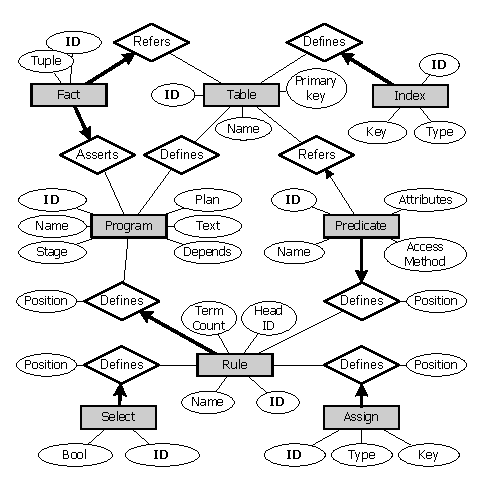
\includegraphics[scale=1.2]{figures/ERDiagram}
\caption{ER Diagram of a query plan in P2.}
\label{ch:evita:fig:p2er}
\end{center}
\end{figure*}

\subsection{Table-izing Optimizer State} 
\label{ch:evita:sec:catalog}

A typical query optimizer maintains a number of data structures to describe the
contents of a query, and to represent the ongoing state of a query planning
algorithm, including fragments (i.e., subplans) of query plans.  Our first task
in designing Evita Raced was to capture this information in a relational
schema.

Figure~\ref{ch:evita:fig:p2er} shows an Entity-Relationship (ER) diagram we
developed that captures the properties of an \OVERLOG program, and its
associated P2 dataflow query plans.  In the figure, entities are {\em squares} with
attributes hanging off of them as {\em ovals}.  An attribute has a name, and if it is
part of the primary key, then it is shown in bold.  Relationships are shown as
{\em diamonds} that include a name description.  Lines connect entities to relationships 
and identify the following constraints.
\begin{itemize}
    \ssp
  \item A bold line indicates the existence of at least one tuple in the output
    of a ``foreign-key join'' with the connecting entities, while a regular line
    imposes no constraints on the ``join'' output.
  \item An arrow directed into a relationship indicates {\em many} tuples from
    the origin entity ``join with'' exactly {\em one} tuple from the entity on
    the other side of the relationship.
\end{itemize}

We derived the constraints in the diagram by reviewing the semantic analysis
rules enforced in the original P2 compiler; we discuss a few of them here for
illustration.  An \OVERLOG~{\em rule} must appear in exactly one {\em program}.
A {\em select} term (e.g., \ol{f\_contains(X,P2) == false} in
Figure~\ref{ch:p2:fig:overlogSP}) is a Boolean expression over attributes in
the predicates of the rule, and must appear in exactly one {\em rule}.  The
diagram indicates that a {\em predicate} must also appear in a unique {\em
rule}, and that it may possibly reference a single {\em table}.  A predicate
that references a table is called a {\em table predicate} (or a
\emph{materialized predicate}), while one that does not reference a table is
called an {\em event predicate}.  An {\em index} is defined over exactly one
{\em table}, and a {\em table} defines at least one index (namely the primary
key index, which P2 always constructs).  Some relations may contain {\em facts}
(input tuples) at startup, each of which must belong to a single program and
must reference a single table.

\begin{figure*}
\ssp
\begin{tabular}{|l|l|p{7cm}|} \hline
{\it Name}& {\it Description} & {\it Relevant attributes} \\ \hline\hline
table     & Table definitions & {\bf table\_id}, primary\_key\\ \hline
index     & Index definitions & {\bf index\_id}, {\bf table\_id}, keys, type \\ \hline
fact      & Fact definitions  & {\bf program\_id}, {\bf table\_id}, {\bf id}, tuple\\ \hline
program   & User program description     & {\bf program\_id}, name, stage, text, depends, plan \\ \hline
rule      & Rules appearing in a program   & {\bf program\_id}, {\bf rule\_id}, name,  term\_count, head\_id \\ \hline
predicate & Relational predicates  & {\bf id}, {\bf rule\_id}, table\_id, name, position, access\_method \\ \hline
select    & Selection predicates  & {\bf id}, {\bf rule\_id}, boolean, position \\  \hline
assign    & Variable substitution statements & {\bf id}, {\bf rule\_id}, variable, value, position \\ \hline 
\end{tabular}
\caption{The Metacompiler Catalog: tables defining an \OVERLOG program and dataflow execution plan.
         The primary key columns are shown in bold. }
\label{tbl:catalog}
\end{figure*}

The conversion from ER diagram to relational format was a textbook
exercise~\cite{DBTextbook}.  Table~\ref{tbl:catalog} lists the set of relations
that capture the entities mentioned in the ER diagram; we refer to this as the
{\em Metacompiler Catalog}.  We modified P2 to create these tables at system
startup, and they are accessible to any \OVERLOG programs (i.e., optimizations)
added to the system.

\subsection{Metacompiler Architecture}
\label{ch:evita:sec:arch}
  
\begin{figure*}[htbp]
\centering
\ssp
\begin{tabular}{|p{2.6cm}|l|p{10cm}|} \hline
{\it Stage name}& {\it Language} & {\it Description} \\ \hline\hline
StageScheduler \text{(Chapter~\ref{ch:evita:sec:stageschedule})} & C++ & 
Coordinates the compilation of stages.\\ \hline
Parser \text{(Chapter~\ref{ch:evita:sec:parser})}  & C++ & 
Bison based parser engineered to populate the Metacompiler Catalog with data from the program AST.\\ \hline
Planner \text{(Chapter~\ref{ch:evita:sec:planner})} & C++ & 
Generates a dataflow description from the program data contained in the Metacompiler Catalog.\\ \hline
Installer \text{(Chapter~\ref{ch:evita:sec:installer})} & C++  & 
Instantiates C++ dataflow objects from a dataflow description. \\ \hline
Delta Rewrite \text{(Chapter~\ref{ch:evita:sec:delta})} & \OVERLOG & 
Converts rules based on materialized tables into an ECA form. \\ \hline
Localization \text{(Chapter~\ref{ch:evita:sec:local})} & \OVERLOG   & 
Rewrites distributed (join) rules into a locally executable form. \\ \hline
Magic-sets \text{(Chapter~\ref{ch:magic})}  & \OVERLOG & 
Rewrites rules to include magic predicates, which act as selection predicates for constants contained in query predicates. \\ \hline
\text{System R} \text{(Chapter~\ref{ch:opt:sec:systemr})} & \OVERLOG  & 
A {\em top-down} dynamic programming optimization. \\ \hline
Cascades \text{(Chapter~\ref{ch:opt:sec:cascades})} & \OVERLOG  & 
A {\em bottom-up} dynamic programming optimization. \\  \hline
\end{tabular} 
\caption{Primary Evita Raced compiler stages. }
\label{tbl:stages}
\end{figure*}
  

Optimization logic expressed in \OVERLOG is declarative, and Evita Raced
realizes this logic by converting it to a dataflow program to be executed by
the P2 dataflow subsystem (Chapter~\ref{ch:p2:sec:p2}).  Here, we describe how
Evita Raced represents query optimization programs as dataflow, and also the
way it orchestrates multiple different optimization programs in P2.

An optimizer built using Evita Raced is composed of an extensible number of
{\em stages}, each of which performs some compilation task on the input
program.  Table~\ref{tbl:stages} describes the primary compiler stages packaged
with the Evita Raced framework.  An Evita Raced stage can be written as a
dataflow program of one or more P2 elements in C++, which are then compiled
into the P2 binary; this is how we implement certain base stages required for
bootstrapping (Chapter~\ref{ch:evita:sec:bootstrap}).  However, the power of
Evita Raced comes from its support for stages written in \OVERLOG.  In addition
to being compactly expressed in a high-level language, \OVERLOG stages can be
loaded into a running P2 installation at any time, without the need to compile
a new P2 binary.

A stage programmer registers a new stage with Evita Raced by inserting a tuple
into the \ol{program} relation.  Such a tuple contains an unique identifier
($program\_id$), a name ($name$), a list of stage dependencies ($depends$ ---
Chapter~\ref{ch:evita:sec:stageschedule}), and the program text ($text$).  The
\ol{program} relation also contains an attribute for the name of the compiler
stage currently operating on the program ($stage$), and the final physical plan
($plan$ --- Chapter~\ref{ch:evita:sec:planner}); these attributes are used to
convey partial compilation results from stage to stage.  We next describe the
interfaces to an Evita Raced compiler stage and how we schedule different
stages when compiling (any) \OVERLOG programs.

\subsubsection{The Stage API}
\label{ch:evita:sec:stages}

An Evita Raced stage can be thought of as a stream query that listens for a
tuple to arrive on an event stream called \ol{<stage>::programEvent}, where
\ol{<stage>} is the name of the stage.  The \ol{<stage>::programEvent} table
contains all the attributes mentioned in the \ol{program} table.  When such a
tuple arrives, the queries that make up that stage execute, typically by
modifying catalog tables in some way.  When a stage competes it inserts a new
\ol{program} tuple, including the current stage name in the $stage$ attribute,
into the program table.

To represent this behavior in a stage written in \OVERLOG, a relatively simple
template can be followed.  An \OVERLOG stage must have at least one rule body
containing the \ol{<stage>::programEvent} predicate.  These stage {\em
initiation} rules react to new programs arriving at the system and trigger
other rules that are part of the same stage.  In addition, the stage must have
at least one rule that inserts a \ol{program} tuple into the \ol{program} table
to signal its completion. 

\subsubsection{Stage Scheduling}
\label{ch:evita:sec:stageschedule}

In many cases, optimization stages need to be ordered in a particular way for
compilation to succeed.  For example, a {\em Parser} stage must run before any
other stages, in order to populate the Metacompiler Catalog.  The {\em Planner}
must follow any query transformation stages, since it is responsible for
translating the (relational) logical query plan into a physical dataflow
representation.  And finally, the {\em Installer} stage must follow the {\em
Planner}, since it instantiates dataflow specifications as P2 C++ elements, and
installs them into the P2 runtime.  

A natural way to achieve such an ordering would be to ``wire up'' stages
explicitly so that predecessor stages directly produce
\ol{<stage>::programEvent} tuples for their successors, in an explicit chain of
stages.  However, it is awkward to modify such an explicit dataflow
configuration upon registration of new stages or precedence constraints.
Instead, Evita Raced captures precedence constraints as {\em data} within a
materialized relation called \ol{StageLattice}, which represents an
order (i.e., an acyclic binary relation) among stages; this partial
order is intended to be a lattice, with the {\em Parser} as the source, and the
dataflow {\em Installer} as the sink.  
 
To achieve the dataflow connections among stages, the built-in {\em
StageScheduler} component (itself a stage) listens for updates to the
\ol{program} table, indicating the arrival of a new \OVERLOG program or the
completion of a compiler stage for an on-going program compilation.  The {\em
StageScheduler} is responsible for shepherding compilation stage execution
according to the \ol{StageLattice}.  Given a \ol{program} update, the
StageScheduler ``joins with'' the \ol{StageLattice} to identify a next stage
that can be invoked, and derives a \ol{<stage>::programEvent} tuple that will
start the given stage; the contents (attributes) of the
\ol{<stage>::programEvent} tuple are the same as those in the updated
\ol{program} tuple.

\begin{figure*}[htbp]
\begin{center}
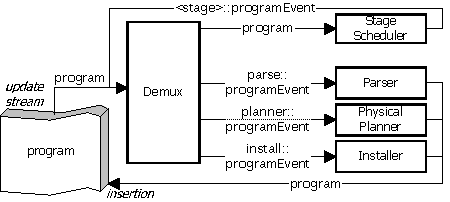
\includegraphics[scale=1.5]{figures/DefaultCompiler}
\ssp
\caption{The Evita Raced (cyclic) dataflow architecture, containing only the 
default compilation stages. The arrows leaving the Demux element
route tuples, based on the tuple name, to the relevant stages on the right.
We focus here on the portion of the P2 dataflow that corresponds 
to the Evita Raced architecture.}
\label{ch:evita:fig:basecompiler}
\end{center}
\end{figure*}

The StageScheduler and any compilation stages (whether built-in or
runtime-installed) are interconnected via the simplified dataflow illustrated
in Figure~\ref{ch:evita:fig:basecompiler}.  The Evita Raced architecture is
embedded in the same P2 dataflow used to execute user queries.  As described in
Chapter~\ref{ch:p2:sec:p2} (and~\cite{p2:sosp}), the dataflow consists of a C++
``demultiplexer'' that routes tuples from its input (on the left) to individual
event handlers listening for particular tuple names.  The Evita Raced runtime
simply adds these ``default stages'' to the bootstrap routine of the P2 system.

Consider the simplicity of how Evita Raced architecture coexists with the P2
dataflow.  To install a new (\OVERLOG) compilation stage into the runtime, the
Installer stage (Chapter~\ref{ch:evita:sec:installer}) simply extends the {\em
Demux} element to include a port for \ol{<stage>::programEvent} tuples, routing
them to the respective rule(s) of a given stage's \OVERLOG program.  The
\ol{StageLattice} relation is also updated (e.g., through fact tuples in the
\OVERLOG stage program) to include its position in the compilation pipeline.
Once installed, the \OVERLOG stage need only follow a simple protocol for when
and how it should execute.

The protocol, followed by stages, indicates when a stage should start (after
receiving a \ol{<stage>::programEvent} tuple) and what it must do on
completion.  When a stage completes, the only requirement is to update the
\ol{program} table with the ``stage'' attribute set to the current stage name.  The
{\em StageScheduler} receives all such updates to the \ol{program} table -- see
Figure~\ref{ch:evita:fig:basecompiler}, the {\em Demux} \ol{program} tuple port
into the {\em StageScheduler} -- and uses the value of the \ol{program}
$depends$ attribute along with the \ol{StageLattice} relation to determine the
next stage.  This covers the full Evita Raced compilation process of an
\OVERLOG program, from the {\em Parser} stage to the {\em Installer} stage, and
any other stages along the way.

To sum up, the lifecycle of a program compilation starts when a user submits a
\ol{program} tuple to the system with a \ol{null} stage attribute.  The
StageScheduler receives that \ol{program} tuple and generates a
\ol{parse::programEvent} tuple (the Parser being the source stage in the
lattice), which is routed by the Demux element to the Parser stage.  When the
Parser is done, it updates that \ol{program} tuple in the corresponding table,
changing the tuple's $stage$ attribute to ``Parser.'' The StageScheduler
receives the \ol{program} tuple, and routes a \ol{planner::programEvent} to the
Demux and eventually the Planner, which goes round the loop again to
the Installer.  Finally, once the Installer is done and notifies the
StageScheduler via a \ol{program} tuple with the $stage$ attribute set to
``Installer,'' the StageScheduler concludes the compilation process.  If the
\OVERLOG program being parsed is itself a new compilation stage, then after
installation, the scheduler updates the stage lattice (e.g., by applying 
stage lattice facts defined in the stage program).


\subsection{Compiler Bootstrapping}
\label{ch:evita:sec:bootstrap}

This section describes the baseline Evita Raced compiler as four simple C++
stages that are loaded by the P2 bootstrap routine.  As in many metaprogramming
settings, this is done by writing a small bootstrap component in a lower-level
language.  Evita Raced is initialized by a small C++ library that constructs
the cyclic dataflow of Figure~\ref{ch:evita:fig:basecompiler}, including the
four default stages shown.  The bootstrap compiler is sufficient to compile
simplified \OVERLOG programs (local rules only, no optimizations) into
operational P2 dataflows.  We describe here the implementation of our Parser,
Planner, and Installer bootstrap stage elements, which form the core foundation
of the Evita Raced architecture.

\subsubsection{Parser}
\label{ch:evita:sec:parser}

The Parser passes the program text it receives in the \ol{parse::programEvent} through
a traditional lexer/parser library specified using flex~\cite{flexUrl} and
bison\cite{bisonUrl}; this library code returns a standard {\em abstract syntax
tree} representation of the text.  Assuming the Parser does not raise an
exception due to a syntax error, it walks the abstract syntax tree, generating
Metacompiler Catalog tuples for each of the semantic elements of the tree.  In
addition to recognizing the different terms of each rule, the parser also
annotates each term with a position, relative to its ``parse'' order.  In
Chapter~\ref{ch:evita:sec:delta}, we will use this position when ``compiling''
a rule into ECA form, and in Chapter~\ref{ch:opt}, we use it to reorder
subgoals in the rule body for optimizing the join order.


\subsubsection{Physical Planner}
\label{ch:evita:sec:planner}

The Planner stage is responsible for doing a na\"{i}ve translation of
Metacompiler Catalog tuples (i.e., a parsed \OVERLOG program) into a dataflow
program.  It essentially takes each rule and deterministically translates it
into a dataflow graph language, based on the rule term positions.

More specifically, for each rule, the Planner considers each term (predicate,
selection or assignment) in order of the position attribute contained in the
relevant Metacompiler Catalog relation.  The predicate representing the event
stream is always planned first, and registers a listener in the Demux element
(recall Figure~\ref{ch:evita:fig:basecompiler}).  The terms following the event
stream are translated, left-to-right, into a C++ dataflow in the same way that
the original P2 system did using select-project-join operator methods.

We further mention three specific details.  First, where the original P2
system translated a logical query plan directly to a software dataflow
structure in C++, we have chosen to create an intermediate, textual
representation of the dataflow.  This representation is in a language akin to
the Click router's dataflow language, but we omit its details here.

Second, unlike the original P2 system, we have introduced a number of new join
methods for in-memory tables.  Prior to this work, P2 only supported
index-nested-loop joins, where the appropriate index was built on the join
column(s) during program compilation.  We have added two elements to the P2
runtime that perform a simple nested-loop join and a sort-merge join on a tuple
from the outer input, with a relation on the inner.  We note that our
sort-merge join is not traditional: it only requires the inner relation to be
sorted.  The P2 architecture does not allow us to sort the outer relation, so
instead we perform a binary search on the inner relation.  The \ol{predicate}
relation contains the choice of join method as one of its attributes, and the
Planner creates the appropriate dataflow element that implements the given join
method.

%% Those are naturally introduced to the P2 physical planner
%% machinery and otherwise
%% creates
%% a listening port in the P2 {\em Demux} on the event stream name. The predicates mentioned in the rule that
%% do not represent the event stream represent lookup operations (joins) on the referenced base relation.
%% A join operator is planned for a predicate by taking the input stream and schema and joining 
%% it - using the $access\_method$ given by the \ol{predicate} tuple - with a base relation producing a new tuple 
%% stream with the join schema. 
%% A selection term plans a filter operator that applies the $boolean$ attribute value to the input 
%% stream and passes only tuples that satisfy this expression to the output stream. \jmh{Again the "plans an operators that does X" doesn't mean much to me.}An assignment term 
%% plans a assignment operator that uses the input stream to evaluate the $value$ attribute (in the \ol{Assign}
%% tuple) to an atomic value. If the input stream contains an attribute named by $variable$ 
%% (in the \ol{Assign} tuple) then the value of that attribute is substituted in the input
%% stream, otherwise a new attribute is added to the input schema with the given value 
%% in the output stream. After all rule body terms have been planned, the planner adds a projection operator
%% that projects the output tuple stream onto the head predicate.

% generates a physical plan for each rule in a program. The execution order of a physical plan in 
% P2 is a leaf-to-root path, with the leaf corresponding to the event predicate and the root being the head 
% predicate. All predicates that lie in between the leaf and the root path are joined against the respective 
% base relation according to the access method given by the predicate tuple. 
% \petros{I would go as far as saying that the physical plan you derive is
% expressed in an operator language reminiscent of the Click
% language. Since we concentrate on logical plan manipulations here we
% don't go into details. The important thing to point out is that whatever
% you do is not tied to a particular runtime; one could take this physical
% plan and install it on a different runtime that isn't our dataflow but
% something else.}

% The initial operator is always the event predicate and it determines when the rule should fire. 
% If the rule does not contain an event predicate then a delta rewrite must be preformed on the rule. 
% The delta rewrite converts the original rule into a set of new rules
% that trigger whenever a side effects\petros{``side affect'' should be
%   ``side effect'' everywhere.} 
% occurs on a table predicate mentioned in the original rule. The delta rewrite is presented 
% in~\cite{boonSigmod}, and we fully adopt this rewrite in our metacompiler. The position attribute 
% defined by each predicate tuple determines the position of the corresponding physical operator in 
% the physical plan. Select and assign operators are also planned at the position indicated by the 
% respective table tuple.

Third, the Planner only understands rules that are in an event-condition-action
(ECA) form.  An \OVERLOG rule may have no event predicate (e.g., ``\ol{table1
:- table2, table3.}'').  A {\em delta rewrite} (from Loo, et
al.~\cite{loo-sigmod06}) is used to convert such rules in an ECA form (E.g.,
``\ol{table1 :- delta\_table2, table3.}'' and ``\ol{table1 :- table2,
delta\_table3.}''.) As in earlier versions of P2~\cite{loo-sigmod06},
\ol{delta\_table} denotes a stream conveying insertions, deletions, or timeout
refreshes to tuples of the target \ol{table}.  We could have done this directly
in the Planner, but instead we built it as an \OVERLOG stage
(Chapter~\ref{ch:evita:sec:delta}).  This decision had an important
consequence; when expressing the delta rewrite stage in \OVERLOG, we had to use
rules that contained an explicit event predicate.  Furthermore, any \OVERLOG
program that contains rules with no explicit event predicate, depends on the
delta rewrite stage.  The delta rewrite stage consists of a mere $12$ \OVERLOG
(ECA) rules ($25$ lines of code), and is one of the first \OVERLOG stages to be
compiled into the system.
 

\subsubsection{Installer}
\label{ch:evita:sec:installer}

Following the Planner stage, what remains is to parse the textual
representation of the physical dataflow, create the corresponding C++ elements,
and ``wire them up'' accordingly.  We have implemented these steps in a single
C++ Installer stage.  Once the elements and their connections are instantiated,
the Installer stage stitches them into the P2 runtime's overall dataflow graph.
In other words, the Installer implemented an extensible dataflow runtime by
dynamically adding new rule instantiations to (possibly new) Demux ports (see
Figure~\ref{ch:evita:fig:basecompiler}); a feature not available prior to the
release of Evita Raced.

% Since our focus here
% is on plan optimization, we omit the engineering
% details of that contribution.
% 



\subsection{Modularity}
\label{ch:evita:sec:modularity}

A stage adds a weak notion of modularity to the \OVERLOG language.  Prior to
Evita Raced, P2 was only able to install a single \OVERLOG program into its
dataflow.  The rules in this program had complete visibility of all
materialized relations, and accordingly side effects to these relations were
visible throughout.  In this work, we had to ensure that side effects made by
one stage were not visible in another, since such overlapping updates against
the Metacompiler Catalog could render it inconsistent.

The first \OVERLOG stage installed into Evita Raced adds stage modularity to
the system.  Itself a rewrite, the stage adds {\em guard} predicates to all
rule bodies in subsequently installed \OVERLOG stages.  These guard predicates
ensure that only rules in an ``active'' stage react to Metacompiler Catalog
updates.  A stage is activated when its \ol{<stage>::programEvent} tuple is
first derived, and deactivated when the stage inserts a finalized \ol{program}
tuple.  Facts added to the \ol{guard} relation activate the rules of a stage,
and deactivate rules in other stages.  We do not mention these guard rules
further since they are completely abstracted way from the programmer.

\subsection{Discussion}

The metacompilation approach of Evita Raced led us to naturally design the
system extensibility around issues of data storage and dataflow, rather than
library loading and control flow modifications.  While rule-based systems are
usually intended to be easier to extend than a procedural system, the internal
implementation of Evita Raced is clean, due to our thorough embrace of the
native dataflow infrastructure, which we use both to execute optimization code,
and orchestrate stages via precedence tables and the StageScheduler cycle.  The
result of this design is that even a major addition to the Evita Raced compiler
entails very minimal modification to the runtime state: only the addition of a
pair of dataflow edges to connect up the new stage, and the insertion of
precedence tuples in a single table.  Beyond the StageScheduler and the four
bootstrap stages, no additional extensibility code was added to P2 to support
Evita Raced.

Despite its simplicity, Evita Raced is flexible enough that other researchers
have used it to enhance P2 with support for new languages at both its input and
output.  First, by extending the Parser element and registering some \OVERLOG
rules, Abadi and Loo were able to get P2 to optimize and rewrite programs
written in a new language, which extends \OVERLOG with the ability to attest to
the provenance of data in a manner similar to that of~\cite{abadi-netdb07}.
Second, Chu, et al. were able to use Evita Raced to cross-compile \OVERLOG programs
into dataflow specifications that execute on the DSN platform, a declarative
networking system that runs on wireless sensor nodes~\cite{chu-sensys07}.


\section{The Delta Rewrite}
\label{ch:evita:sec:delta}

In this section we describe our declarative implementation of the delta rewrite
for \OVERLOG rules.  The rewrite itself consists of only $12$ rules, which
includes rules for stage activation, finalization and general housekeeping of
the Metacompiler Catalog relations.  Before diving into the specific rules for
the rewrite, we describe its actions by example.

\subsection{Delta by Example}

\begin{figure*}[!t]
\ssp
\centering
\begin{lstlisting}
materialize(link, infinity, infinity, keys(1,2)).
materialize(path, infinity, infinity, keys(1,2,3)).
materialize(shortestPath, infinity, infinity, keys(1,2,3)).
  
r1 path(@X, Y, P, C) :- 
   link(@X, Y, C), P := f_cons(X, Y).

r2 path(@X, Z, P, C) :-
   link(@X, Y, C1), 
   path(@Y, Z, P2, C2),
   f_contains(X, P2) == false,
   P := f_cons(X, P2), C := C1 + C2.

r3 minCostPath(@X, Y, a_min<C>) :-
   path(@X, Y, P, C).

r4 shortestPath(@X, Y, P, C) :-
   minCostPath(@X, Y, C), 
   path(@X, Y, P, C).

\end{lstlisting}
\caption{\label{ch:evita:fig:basicSP}Shortest path program.}
\end{figure*}

Consider the shortest path program in Figure~\ref{ch:evita:fig:basicSP}: copied
over from Figure~\ref{ch:p2:fig:overlogSP}.  First thing to notice is the {\bf
materialize} statements at the top.  They indicate that positive lifetime
tables should exist for \ol{link}, \ol{path}, and \ol{shortestPath} tuples,
along with the appropriate primary key columns.  Since there is no {\bf
materialize} statement for the \ol{minCostPath} predicate, P2 considers such
tuples to be events, that will end up triggering rule~\ol{r4} when ``pulled''
from the event queue.  The question then is, what triggers the other rules to
produce \ol{minCostPath} event tuples?

\begin{figure*}[!t]
\ssp
\centering
\begin{lstlisting}
materialize(link, infinity, infinity, keys(1,2)).
materialize(path, infinity, infinity, keys(1,2,3)).
materialize(shortestPath, infinity, infinity, keys(1,2,3)).

r1 path(@X, Y, P, C) :-
   %*$\Delta$*)link(@X, Y, C), 
   P := f_cons(X, Y).

r2a path(@X, Z, P, C) :-
    %*$\Delta$*)link(@X, Y, C1), 
    path(@Y, Z, P2, C2),
    f_contains(X, P2) == false,
    P := f_cons(X, P2), C := C1 + C2.

r2b path(@X, Z, P, C) :-
    %*$\Delta$*)path(@Y, Z, P2, C2), 
    link(@X, Y, C1),
    f_contains(X, P2) == false,
    P := f_cons(X, P2), C := C1 + C2.

r3 minCostPath(@X, Y, a_min<C>) :-
   %*$\Delta$*)path(@X, Y, P, C).

r4 shortestPath(@X, Y, P, C) :-
   minCostPath(@X, Y, C), 
   path(@X, Y, P, C).
\end{lstlisting}
\caption{\label{ch:evita:fig:basicSPDelta}Delta rewrite rules from Figure~\ref{ch:evita:fig:basicSP}.}
\end{figure*}

The delta rewrite converts the rules in Figure~\ref{ch:evita:fig:basicSP} into
the rules shown in Figure~\ref{ch:evita:fig:basicSPDelta}.  The {\em new} rules
contain a single $\Delta$ predicate, shown (by convention) at the front of the
rule.  Since rule~\ol{r4} already contains an {\emph event} predicate, the
delta rewrite simply ignores this rule, which is fixed to trigger off of
\ol{minCostPath} tuples.  The remaining rules are converted into $\Delta$ form
so that they can be installed into the P2 runtime by the $Planner$ stage.  We
start with rule~\ol{r1}, which contains the single subgoal \ol{link}.  The
delta rewrite simply adds a delta annotation to this predicate, informing the
$Planner$ to trigger the rule when a receive/insert/delete event occurs on the
\ol{link} relation.  The same thing happens in rule~\ol{r3} w.r.t., the
\ol{plan} relation.

Rule~\ol{r2} has two subgoals \ol{link} and \ol{path}, both of which are
materialized tables.  In this case, we must break the rule into two disjoint
rules (one for each materialized subgoal).  The first of these rules will
trigger on (say) the \ol{link} tuple, followed by a join with \ol{path}, etc.
The second rule triggers on \ol{path} event tuples, and joins with the
\ol{link} relation, etc.  Both of these rules project onto the \ol{path}
relation, which in turn triggers further invocations of rule~\ol{r2b} on new
\ol{path} data.

\subsection{Declarative Delta}

\begin{figure*}[!t]
\ssp
\centering
\begin{lstlisting}
%* /* Initiate a rewrite at position $1$ of a rule not already containing an event *)
%*    predicate in this position. */ *)
d1 rewrite(@A, Pid, Rid, PredID, f_idgen(), f_idgen(), Pos) :-
   delta::programEvent(@A, Pid, ...), 
   sys::rule(@A, Rid, Pid, _, HeadID, _, _, _, Goals),
   sys::predicate(@A, PredID, Rid, _, Name, Tid, _, Schema, Pos),
   Tid != null, Pos == 1.

%* /* Initiate a rewrite position for each predicate in the rule body. */ *)
d2 rewrite(@A, Pid, Rid, PredID, f_idgen(), f_idgen(), Pos) :-
   rewrite(@A, Pid, Rid, ...),
   sys::predicate(@A, PredID, Rid, ..., Schema, Pos),
   Pos > 1.
\end{lstlisting}
\caption{\label{ch:evita:fig:delta1}Deduce a rewrite fact for a new delta rule to be
created for a particular table predicate in the original rule's body.}
\end{figure*}

We now turn to the delta rewrite \OVERLOG stage; used translate
Figure~\ref{ch:evita:fig:basicSP} into Figure~\ref{ch:evita:fig:basicSPDelta}.
Prior to the installation of this stage, only rules containing an explicit
event predicate can be installed.  As a result, all rules described here
contain an explicit event predicate e.g., the \ol{delta::programEvent} tuple.

Figure~\ref{ch:evita:fig:delta1} contains two rules that initiate the delta
rewrite by deducing a rewrite tuple from each rule in the target program.
Rule~\ol{d1} triggers on the \ol{delta::programEvent} tuple and ``joins with''
the \ol{rule} and \ol{predicate} tables, selecting out the predicate in
position~$1$.  Recall that this is the event position, and that this rewrite
ignores rules containing an explicit event.  Therefore, if the predicate in
position~$1$ references a materialized table ($Tid\ !=\ null$) --- it is not an
event --- then we need to rewrite it.  Once a \ol{rewrite} event tuple has been
deduced for a given target rule, rule~\ol{d2} initiates a second \ol{rewrite}
event tuple for each predicate in the target rule's body.  The $Pos > 1$
selection avoids the head predicate (position $0$) and the first predicate
already handled by rule~\ol{d1}.

\begin{figure*}[!t]
\ssp
\centering
\begin{lstlisting}
%* /* Put the delta predicate in the first position of the new rule. */ *)
d3 sys::predicate(@A, f_idgen(), NewRid, Notin, Name, Tid, "DELTA", 
                  Schema, 1) :-
   rewrite(@A, Pid, Rid, DeltaPredID, NewRid, NewHeadID, _),
   sys::predicate(@A, DeltaPredID, Rid, Notin, Name, Tid, ECA, 
                  Schema, Pos).

%* /* Make a new head predicate for the new rule by copying the old head predicate. */ *)
d4 sys::predicate(@A, NewHeadID, NewRid, Notin, Name, Tid, ECA, 
                  Schema, 0) :-
   rewrite(@A, Pid, Rid, DeltaPredID, NewRid, NewHeadID, _),
   sys::rule(@A, Rid, Pid, _, HeadID, ...),
   sys::predicate(@A, HeadID, Rid, Notin, Name, Tid, ECA, Schema, _).
\end{lstlisting}
\caption{\label{ch:evita:fig:delta2}Rules that copy the old head predicate from the old rule
to the new rule, and creates the delta predicate in the new rule from the subgoal referenced
by the rewrite tuple.}
\end{figure*}

Assume we have initiated a rewrite tuple for a given rule $r$ and body
predicate $p_i$ at position~$i$.  The next step is to actually create the new
rule $\Delta r_i$ with predicate $\Delta p_i$ that references the delta events of
predicate $p_i$.  The new rule will take the following form $h$~\ol{:-}~$\Delta
p_i, G_{j!=i}$, where $h$ references the original head predicate in rule $r$
and $G_{j!=i}$ is the list of subgoals that exclude predicate~$p_i$.

Figure~\ref{ch:evita:fig:delta2} contains two rules that create the head
predicate ($h$) and the delta predicate ($\Delta p_i$) for the new delta rule
($\Delta r_i$).  Rule~\ol{d3} specifically creates the delta predicate, placing
it in position~$1$ (by convention) of the new rule.  Next, rule~\ol{d4} copies
the head predicate, from the old rule, by joining the old rule identifier
($Rid$) in \ol{rewrite} with the \ol{rule} table, and the \ol{predicate} table
along the old head predicate identifier ($HeadID$).  The new head predicate is
given a new predicate identifier ($NewHeadID$) and the new rule identifier
($NewRid$).


\begin{figure*}[!t]
\ssp
\centering
\begin{lstlisting}
%* /* Kick off an iterator for the remaining rule subgoals. */ *)
d5 remainder(@A, Pid, Rid, NewRid, 1, 2, Pos) :-
   rewrite(@A, Pid, Rid, DeltaPredID, NewRid, _, Pos).

%* /* Forward the remainder iterator along the subgoals. */ *)
d6 remainder(@A, Pid, Rid, NewRid, OldPos+1, NewPos, DeltaPos) :-
   remainder(@A, Pid, Rid, NewRid, OldPos, NewPos, DeltaPos),
   sys::rule(@A, Rid, Pid, ..., Goals),
   OldPos < Goals,
   NewPos := OldPos == DeltaPos ? NewPos : NewPos + 1.

%* /* Copy table predicate to the new delta rule. */ *)
d7 sys::predicate(@A, f_idgen(), NewRid, Notin, Name, Tid, null, 
                  Schema, NewPos) :-
   remainder(@A, Pid, Rid, NewRid, OldPos, NewPos, DeltaPos),
   sys::predicate(@A, PredID, Rid, Notin, Name, Tid, _, Schema, OldPos),
   OldPos != DeltaPos.

%* /* Make a new assignement for the new delta rule. */ *)
d8 sys::assign(@A, f_idgen(), NewRid, Var, Value, NewPos) :-
   remainder(@A, Pid, Rid, NewRid, OldPos, NewPos, _),
   sys::assign(@A, Aid, Rid, Var, Value, OldPos).

%* /* Make a new selection for the new delta rule. */ *)
d9 sys::select(@A, f_idgen(), NewRid, Bool, NewPos) :-
   remainder(@A, Pid, Rid, NewRid, OldPos, NewPos, _),
   sys::select(@A, Sid, Rid, Bool, OldPos, AM).

\end{lstlisting}
\caption{\label{ch:evita:fig:delta3}Rules that copy old subgoals to the new 
delta rule.}
\end{figure*}

Figure~\ref{ch:evita:fig:delta3} contains the next group of rules that copy the
body predicates $G_{j!=i}$ from the old rule $r$ to the new $\Delta r_i$ rule,
excluding predicate $p_i$.  We express this through a secondary group of event
tuples, called \ol{remainder}, that reference each body predicate in rule $r$
excluding $p_i$.  A \ol{remainder} tuple contains the predicate position
relative to rule $r$ and a new position in the $\Delta r_i$ rule.  The new
position must start at $2$, following the delta predicate, which is already set
to $p_i$.

Rule~\ol{d5} initiates the first \ol{remainder} tuple from a \ol{rewrite}
tuple, and rule~\ol{d6} carries further \ol{remainder} deductions along each
subgoal in the body of rule $r$.  A \ol{remainder} tuple contains three
attributes that reference rule positions; shown here by the $OldPos$, $NewPos$
and $DeltaPos$ variable names.  The $OldPos$ variable specifies the predicate
position to copy from the original rule to the new $\Delta$ rule, and $NewPos$
is its position in this new rule.  The $DeltaPos$ variable refers to the
position of $p_i$, the new $\Delta$ predicate, in the original rule.  Special
logic is used to avoid predicate $p_i$ w.r.t., \ol{remainder} tuples.  For
example, rule~\ol{d6} does not increment the $NewPos$ when $OldPos\ ==\
DeltaPos$.  The remaining rules (\ol{d7}, \ol{d8} and \ol{d9}) deal with
copying subgoals rule~$r$ to the new $\Delta r_i$ rule.  Notice that rule~\ol{d7}
skips predicate $p_i$ at position $DeltaPos$.

\begin{figure*}[!t]
\ssp
\centering
\begin{lstlisting}
%* /* Create the new rule */ *)
d10 sys::rule(@A, NewRid, Pid, Name, NewHeadID, null, Delete, Goals) :-
    rewrite(@A, Pid, Rid, DeltaPredID, NewRid, NewHeadID, Pos),
    sys::predicate(@A, DeltaPredID, Rid, _, PredName, ...),
    sys::rule(@A, Rid, Pid, RuleName, _, _, Delete, Goals),
    Name := RuleName + "delta" + PredName + Pos.

%* /* Clean up old rule state */ *)
d11 delete sys::rule(@A, Rid, Pid, Name, HeadID, P2DL, Delete, Goals) :-
    rewrite(@A, Pid, Rid, ...),
    sys::rule(@A, Rid, Pid, Name, HeadID, P2DL, Delete, Goals).
  
%* /* Signal the completion of the delta rewrite to the $StageScheduler$. */ *)
d12 sys::program(@A, Pid, Name, Rewrite, "delta", Text, Msg, 
                 P2DL, Src) :-
    programEvent(@A, Pid, Name, Rewrite, Status, Text, Msg, P2DL, Src).
\end{lstlisting}
\caption{\label{ch:evita:fig:delta4}Creates a new rule tuple that references the delta 
rewrite rule. Cleans up the old (non-delta) rule. Inserts a program tuple indicating
that the delta rewrite has finished. }
\end{figure*}

The final set of rules shown in Figure~\ref{ch:evita:fig:delta4} perform
housekeeping tasks related to this rewrite.  Rule~\ol{d10} creates a rule tuple
that references the delta rule $\Delta r_i$ for a given delta predicate $\Delta
p_i$.  The old rule~$r$ is deleted in rule~\ol{d11}, which, through
materialized view maintenance, removes the old head predicate and subgoals.
Finally, rule~\ol{d12} inserts a \ol{program} tuple that indicates the
completion of the delta rewrite stage.~\footnote{Note that this entire rewrite
is performed in a single P2 {\em dataflow} fixpoint.}

\section{The Localization Rewrite}
\label{ch:evita:sec:local}

\begin{figure*}[!t]
\ssp
\centering
\begin{lstlisting}
r2a link_copy(@Y, X, Y, C1) :-
    link(@X, Y, C1).

r2b path(@X, Z, P, C) :-
    link_copy(@Y, X, Y, C1), 
    path(@Y, Z, P2, C2),
    f_contains(X, P2) == false,
    P := f_cons(X, P2), C := C1 + C2.
\end{lstlisting}
\caption{\label{ch:evita:fig:basicSPLocal}The localized version of rule~\ol{r2} in
Figure~\ref{ch:evita:fig:basicSP}.}
\end{figure*}

We briefly describe the localization compiler stage, which turns a rule with
multiple location specifiers in its body, into many rules, each of which has a
single location specifier in its body; turning a distributed join into a set of
local joins with partial result transmissions among the rules
involved~\cite{loo-sigmod06}.  This rewrite was part of the original P2 system,
but implemented in C++ and woven into the monolithic compiler.  In Evita Raced,
the localization rewrite stage contained $11$ rules that resembled the rules in
the delta rewrite stage.  Therefore, we provide a high level description of
this rewrite, and its declarative structure.

We start with an example description using rule~\ol{r2} from
Figure~\ref{ch:evita:fig:basicSP}.  This rule is rewritten into the two rules
shown in Figure~\ref{ch:evita:fig:basicSPLocal}.  The \ol{link\_copy} (event)
predicate forwards \ol{link} tuples at node $X$ to node $Y$.  This will result
in a network transfer of \ol{link} tuples $@X$ to \ol{link\_copy} tuples $@Y$.
At node $Y$, the \ol{link\_copy} tuples trigger rule~\ol{r2b}, which completes
the execution of rule~\ol{r2} before sending the \ol{path} results back to
node~$X$.

Declaratively, the localization stage traverses distributed rules in
left-to-right order; rules with local-only body predicates are selected out
early in the stage.  The location attribute of the current predicate in this
traversal is stored along with the cursor information of the traversal.  A
\ol{rewrite} is derived if the traversal reaches a predicate with a location
attribute that differs from the previous.  The \ol{rewrite} tuple {\em splits}
the rule at the given position, creating a new {\em glue} predicate $IR\_copy$,
and two new rules defined as follows.
\begin{CompactEnumerate} 
\item {\bf IR\_copy} :- (predicates to the left, excluding the \ol{rewrite} position).  
\item (original rule head predicate) :- {\bf IR\_copy}, (predicates to the right, including
  the \ol{rewrite} position).  
\end{CompactEnumerate} 
The location attribute in the {\bf IR\_copy} predicate is taken from the
predicate at the \ol{rewrite} position.  That is, the predicate with the
``new'' location attribute.  The other attributes in the {\bf IR\_copy}
predicate are taken from the predicates to the left of (and not including) the
\ol{rewrite} position, which represents the schema of the intermediate result
({\bf IR\_copy}).  The algorithm then removes the original rule, and moves
recursively on to the second rule, which contains the remaining body predicates
that need to be searched (and possibly split).  The recursion terminates at the
rightmost predicate position.

\section{Summary} 
\label{ch:evita:sec:summary} 

The delta and localization stages are program rewrites necessary to make
materialized (no event predicate) and distributed rules executable.  These
rewrites are expressed compactly in \OVERLOG (around 12 rules each), and
avoid complex C++ code in the $Planner$ stage implementation.  The original
P2 code that performed these tasks consisted of a few hundred lines of code
spread throughout the system implementation; making it hard to evolve.

The Evita Raced metacompilation framework allows \OVERLOG compilation tasks to
be written in \OVERLOG and executed in the P2 runtime engine.  It provides
significant extensibility via a relatively clean declarative language.  As we
will see next, many of the tasks of query optimization -- dynamic programming,
dependency-graph construction and analysis, statistics gathering -- appear to
be well served by a recursive query language.  The notion of metacompilation
also leads to a very tight implementation with significant reuse of code needed
for runtime processing.



